\documentclass[10pt]{article}
\label{articlepackage}

%\usepackage{tgbonum}
\usepackage{soul}
%\usepackage{hyperref}
\usepackage{multicol}

\usepackage{setspace}
\usepackage{slashed}
%\doublespacing

\usepackage[T1]{fontenc}
\usepackage{ifthen}
\usepackage{mathrsfs}


\usepackage{bm}
\usepackage{bibentry}
\usepackage{subcaption}
\usepackage{wrapfig}
\usepackage{amsmath}
\numberwithin{equation}{section}
\numberwithin{figure}{section}
\numberwithin{table}{section}
\numberwithin{footnote}{section}
\usepackage{mathtools}
\usepackage[inline]{enumitem}
\usepackage{booktabs}
%\usepackage[usenames,dvipsnames,pdftex]{xcolor}
\usepackage{tikz}
\usetikzlibrary{backgrounds,shapes,arrows,positioning,calc,snakes,fit}
\usepgflibrary{decorations.markings}
\usepackage{framed}

% \setcounter{section}{-1}

\usepackage{graphicx} % standard package
\usepackage{todonotes} % standard package
\usepackage{amsmath} % standard package
\DeclareMathOperator{\sech}{sech}
\newcommand*\diff{\mathop{}\!\mathrm{d}}
\newcommand{\txtd}{\textrm{d}}
\usepackage{amssymb} % useful for double backed letter functions
%%%%%%%%%%%%%%%%%%%%%%%%%%%%%%%%%%%%
\usepackage{amsthm} % used to define theorem objects with command \begin{theorem} etc.
\newtheorem{theorem}{Theorem}[section]
\newtheorem{example}{Example}[subsection]
\newtheorem*{definition}{Definition}
%%%%%%%%%%%%%%%%%%%%%%%%%%%%%%%%%%%%
\usepackage[numbers, sort&compress]{natbib}
\bibliographystyle{apsrev} % bibliography package and style
\renewcommand{\bibfont}{\small}
\renewcommand{\citenumfont}[1]{\textbf{#1}}
\renewcommand{\bibnumfmt}[1]{[\color{darkblue}\textbf{#1}\color{black}]}
%%%%%%%%%%%%%%%%%%%%%%%%%%%%%%%%%%%%
\usepackage{listings} % code listing and options
\usepackage{color}
%New colors defined below
\definecolor{codegreen}{rgb}{0,0.6,0}
\definecolor{codegray}{rgb}{0.5,0.5,0.5}
\definecolor{codepurple}{rgb}{0.58,0,0.82}
\definecolor{backcolour}{rgb}{0.95,0.95,0.92}
%Code listing style named "mystyle"
\lstdefinestyle{mystyle}{
  backgroundcolor=\color{backcolour},   commentstyle=\color{codegreen},
  keywordstyle=\color{magenta},
  numberstyle=\tiny\color{codegray},
  stringstyle=\color{codepurple},
  basicstyle=\footnotesize,
  breakatwhitespace=false,
  breaklines=true,
  captionpos=b,
  keepspaces=false,
  numbers=right,
  numbersep=4pt,
  showspaces=false,
  showstringspaces=false,
  showtabs=false,
  tabsize=2
}
\lstset{style=mystyle}

\usepackage{tensor}

\usepackage{color}
\definecolor{SAEblue}{rgb}{0, .62, .91}
\definecolor{linkgreen}{RGB}{11, 102, 35}
\definecolor{darkblue}{rgb}{.11, .102, .35}

\usepackage{sectsty}
\sectionfont{\color{darkblue}\centering \large \textsc}
\subsectionfont{\color{darkblue}\centering \normalsize \textit}
\subsubsectionfont{\color{darkblue}\centering \small \textit}
\renewcommand\thesection{\Roman{section}}
\renewcommand\thesubsection{\arabic{section}.\arabic{subsection}}

\renewcommand\theequation{{\color{SAEblue}\arabic{section}.\arabic{equation}}}
\usepackage[colorlinks]{hyperref}
\hypersetup{colorlinks=true, urlcolor=black, citecolor=linkgreen, runcolor=black, menucolor=black, filecolor=black, anchorcolor=black, linkcolor=black}
\theoremstyle{definition}

\renewcommand\vec{\mathbf}
\newcommand{\normord}[1]{\raisebox{0.5pt}{:}\,#1\,\raisebox{0.5pt}{:}}
\newcommand{\dagg}{^{\dagger}}
\newcommand{\pr}{^{\prime}}
\newcommand{\nhat}{\hat{\bm{n}}}
\newcommand{\hamilt}{\mathcal{H}}
\newcommand{\mA}{\mathcal{A}}
\newcommand{\mW}{\mathcal{W}}
\newcommand{\mN}{\mathcal{N}}
\newcommand{\mD}{\mathcal{D}}
\newcommand{\mS}{\mathcal{S}}
\newcommand{\mL}{\mathcal{L}}
\newcommand{\mC}{\mathcal{C}}
\newcommand{\mO}{\mathcal{O}}
\newcommand{\mM}{\mathcal{M}}
\newcommand{\mT}{\mathcal{T}}
\newcommand{\mZ}{\mathcal{Z}}
\newcommand{\mR}{\mathcal{R}}
\newcommand{\II}{\mathbb{I}}
\newcommand{\RR}{\mathbb{R}}
\newcommand{\ZZ}{\mathbb{Z}}
\newcommand{\CC}{\mathbb{C}}
\newcommand{\FF}{\mathbb{F}}
\newcommand{\lie}[1]{\mathcal{L}\left(#1\right)}
\newcommand{\set}[1]{\left\{#1\right\}}
\newcommand{\SO}[1]{\textrm{SO}\left(#1\right)}
\newcommand{\SU}[1]{\textrm{SU}\left(#1\right)}
\newcommand{\Orth}[1]{\textrm{O}\left(#1\right)}
\newcommand{\Uni}[1]{\textrm{U}\left(#1\right)}
\newcommand{\paraskip}{\vspace{10pt}}
\newcommand{\del}{\partial}
\newcommand{\TeG}{\mathcal{T}_e(\mathscr{G})}
\newcommand{\TpM}{\mathcal{T}_p(\mathcal{M})}
\newcommand{\TpMs}{\mathcal{T}^{\star}_p(\mathcal{M})}
\newcommand{\etamn}[1]{\eta#1{\mu \nu}}
\newcommand{\upd}[1]{\text{d}#1 \,}
\newcommand{\ud}{\text{d}}
\newcommand{\group}{\mathscr{G}}
\newcommand{\alge}{\mathfrak{g}}
\newcommand{\twobytwo}[4]{\begin{pmatrix}#1&#2 \\ #3&#4 \end{pmatrix}}
\newcommand{\thrbythr}[3]{\begin{pmatrix}#1 \\ #2 \\ #3\end{pmatrix}}
\newcount\colveccount
\newcommand*\colvec[1]{
        \global\colveccount#1
        \begin{pmatrix}
        \colvecnext
}
\def\colvecnext#1{
        #1
        \global\advance\colveccount-1
        \ifnum\colveccount>0
                \\
                \expandafter\colvecnext
        \else
                \end{pmatrix}
        \fi
}

\usepackage[flushmargin, hang]{footmisc}
  \addtolength{\footnotesep}{1mm}
  \setlength{\footnotemargin}{1em}
  \renewcommand{\thefootnote}{\tiny\textbf{\arabic{section}.\arabic{footnote}}}
  \renewcommand\footnoterule{{\hrule height 0.2pt}}

\captionsetup[figure]{labelsep=quad, labelfont=bf, textfont=it, width=0.8\linewidth}
\renewcommand\thefigure{\arabic{section}.\arabic{figure}}

\newenvironment{Figure}
  {\par\medskip\noindent\minipage{\linewidth}}
  {\endminipage\par\medskip}

\newcommand{\Abs}[1]{\left| #1 \right|}
\newcommand{\tr}{\text{Tr}}

\renewcommand\labelitemi{\raisebox{0.25ex}{\tiny$\bullet$}}
\setenumerate{label=\color{SAEblue}{\textbf{\arabic*}}\color{black})}


\usepackage[most]{tcolorbox}
\newtcolorbox{titlebox}{arc=0mm,auto outer arc, colback=blue!5!white,colframe=black!75!black,leftrule=0pt,rightrule=0pt,toprule=1pt,bottomrule=1pt}

\newtcolorbox{subbox}{arc=0mm,auto outer arc, colback=white!5!white,colframe=black!75!black,leftrule=0pt,rightrule=0pt,toprule=0pt,bottomrule=1pt}

\newtcolorbox{examplebox1}{breakable,enhanced,arc=0mm,auto outer arc, colback=black!5!white,colframe=black!75!black,leftrule=1pt,rightrule=0pt,toprule=0pt,bottomrule=0pt,left=0mm,right=0mm}

\newtcolorbox{examplebox2}{breakable,enhanced,arc=0mm,auto outer arc, colback=white!5!white,colframe=black!75!black,leftrule=1pt,rightrule=0pt,toprule=0pt,bottomrule=0pt,left=0mm,right=0mm}

\usepackage{todonotes}
\newcommand{\mytodo}[1]{\todo[bordercolor=white, color=SAEblue!40!white]{\small #1}}

\usepackage{tocloft}

%\renewcommand\cftsecfont{\normalsize \scshape}
%\renewcommand\cftsecpagefont{\normalsize \itshape}
\renewcommand\cftsubsecfont{\small}
\renewcommand\cftsubsecpagefont{\small}
\renewcommand\cftsubsubsecfont{\small \itshape}
\renewcommand\cftsubsubsecpagefont{\small}
%\setuptodonotes{fancyline, color=linkgreen!30}

\usepackage{tocloft}
\usepackage[labelfont=bf]{caption}
\makeatletter
\renewcommand{\@cftmaketoctitle}{}
\makeatother

\usepackage[margin=0.8in]{geometry}
%\usepackage[margin=1.2in]{geometry}
\usepackage{fancyhdr}
\pagestyle{fancy}
\lhead{\small\textsc{Filling in the Details}}
\chead{}
\rhead{}
\lfoot{}
\cfoot{\texttt{\thepage}}
\rfoot{}

\renewcommand*{\thefootnote}{\fnsymbol{footnote}}
\setcounter{footnote}{1}

\begin{document}
\hrule
\vspace{1pt}
\hrule
\begin{center}
\large\textsc{\color{darkblue}\textbf{Scalar Dark Matter and Neutrino Masses: Filling in the Gaps}}
\vspace{5pt}

\footnotesize\textit{\textbf{J.B.G. Alvey}, Theoretical Particle Physics and Cosmology, King's College London\footnote{\href{mailto:james.alvey@kcl.ac.uk}{james.alvey@kcl.ac.uk}}}
\end{center}
\begin{abstract}
\noindent This report fills in the majority of the technical details associated with the analysis. These include (i) information regarding the TXS $0506$+$056$ blazar and the $290\,\text{TeV}$ neutrino event, (ii) a luminosity analysis at these high energies to support the choice of mean free path, (iii) a consideration as to including the mass hierarchy of neutrinos, and, (iv) details regarding the cross section in the real and complex cases.
\end{abstract}
\hrule
\tableofcontents
\vspace{5pt}
\hrule
\vspace{1pt}
\hrule
\vspace{10pt}
%\begin{multicols}{2}
\renewcommand{\thefootnote}{\tiny\textbf{\arabic{section}.\arabic{footnote}}}
\section{Introduction}
In summary of the state of the work done so far, the following has been considered;
\begin{enumerate}
  \item \textit{Cross-Section:} Computed the cross section for the process $\nu_i\nu_j \rightarrow \delta \delta$, which holds in both the real and complex cases.
  \item \textit{Constraints on the Effective Theory:} Presented a literature review on the constraints on the couplings and masses within the effective theory, as well as presenting our own interpretation of the steps to get there; for example in the computation of the loop integral for the neutrino mass.
  \item \textit{UV Theories:} Discussed the possible UV embeddings of the effective theory and motivated how they link neutrino mass generation and dark matter.
\end{enumerate}
In order to take the project further, we need to fill in some of the details regarding how to improve on the constraints presented in the review paper. This requires a deeper analysis of the TXS $0506$+$056$ blazar, and the high energy neutrino event. This includes extending the luminosity analysis to the PeV scale, as well as collecting some data regarding the energies and uncertainties. This will be used to justify our method of using the mean free path to constrain the model.

We also need to clarify some assumptions regarding which processes contribute to the cross-section, and justify why we neglect some channels. Finally, we consider how to include the possible mass hierarchies in the neutrino sector within the model.
\section{IceCube and IceCube-$170922$A}
\subsection{The IceCube Detector}
The IceCube neutrino observatory \cite{IceCube} is located at the South Pole, consisting of one cubic kilometre of Antarctic ice. The goal of the project is to detect very high energy neutrinos from astrophysical sources. In this regard it is sensitive to energies in the range $300\,\text{TeV}$ to $1\,\text{EeV}$. The important specifics of the design are that it is a Cherenkov detector. When a neutrino enters the ice, a muon is produced which emits Cherenkov radiation as it propagates through the medium. The energy of this muon, $\hat{E}_\mu$ is measured along with the propagation path. This can then be used to reconstruct;
\begin{itemize}
  \item The neutrino energy, $E_\nu$, from the muon energy prior, $\hat{E}_\mu$ via for example Figure S5 in \cite{IceCube2018}. As a reference, in \cite{Kelly}, an estimated fit is given which can be used in simple practical cases;
  \begin{equation}
    \left(\frac{E_\nu}{\textrm{TeV}}\right) = 1.92\left(\frac{\hat{E}_\mu}{\textrm{TeV}}\right)^{1.14}
  \end{equation}
  \item The declination and right ascension of the original neutrino path.\footnote{One can access this data \href{https://icecube.wisc.edu/science/data/access}{\textit{here}}.} This is vital in matching up events with possible sources, and has lead to the deduction that the neutrino events we will be interested were most likely sourced from a blazar, TXS $0506$+$056$, at a redshift of $z \simeq 0.3365$.
\end{itemize}
\subsection{TXS $0506$+$056$}
As discussed above, the IceCube experiment is searching for high energy astrophysical neutrinos. Only very particular types of astrophysical object can produce such energetic particles. Of particular interest to us are objects known as \textit{blazars}. These are \textit{Active Galactic Nuclei (AGN)}, which consist of a supermassive black hole that converts the gravitational and rotational energy of accreting matter into highly relativistic jets \cite{Ackermann2018} pointing in our direction. In particular, IceCube believes to have detected high energy neutrinos from a known $\gamma$-ray source TXS $0506$+$056$. The key fact regarding this blazar is that it is at a redshift \cite{Kelly};
\begin{framed}
\begin{equation}
  z_{\mathrm{TXS}} \simeq 0.3365 \Rightarrow d_{\mathrm{TXS}} \simeq 1.3 \, \textrm{Gpc}
\end{equation}
\end{framed}
\noindent where $d_{\mathrm{TXS}}$ is the comoving distance to the blazar.\footnote{$1\,\textrm{Gpc} \simeq 3.08567 \times 10^{27} \, \textrm{cm}$} This therefore presents a very interesting regime in which to test fundamental physics: we have $\textrm{TeV}$ - $\textrm{PeV}$ energy neutrinos propagating across gigaparsecs of distance. Along the way, we can therefore consider interactions with dark matter, the cosmic neutrino background etc. As we shall discuss further below, it also presents a prime example of the utility of \textit{multimessenger astronomy} \cite{Kellya, Ackermann2018} where neutrino events are calibrated with other $\gamma$ and X-ray experiments such as Fermi-LAT, H.E.S.S., and the Swift XRT.

To understand the relationship between the flaring $\gamma$-ray source TXS $0506$+$056$ and IceCube, one should note that on $22$ Septemeber $2017$, a neutrino with an energy of $\sim 290\,\textrm{TeV}$ was observed at IceCube (IceCube-$170922$A). This prompted a couple of responses;
\begin{itemize}
  \item \textit{Multimessenger Approach:} Immediately after the event, multiple collaborations began to establish the coincidence of the neutrino alert with the flaring state of TXS $0506$+$056$. Broadly this relies on correlating $\gamma$-ray and X-ray measurements of known catalogs of astrophysical objects with the angular position of the reconstructed neutrino path. For a more detailed account of this, see \cite{Ackermann2018}, however the salient point is that the chance coincidence is currently ruled out at $3-3.5\sigma$.
  \item \textit{Historical Approach:} It also provoked a search into data taken in $2014-15$ where it was found that $13 \pm 5$ excess events \cite{Kelly} appear to \textit{also} be coincident with TXS $0506$+$056$ in its flaring state. It thus appears that this blazar is a source of high energy astrophsyical neutrinos. The discussion of the nature of this historical event is discussed more in \cite{Kelly}, where the author makes use of the available data to constrain secret interactions of neutrinos.
\end{itemize}
We will be interested in the high energy event to place our own constraints on the model under consideration. To end this section, we note the careful analysis in \cite{Ackermann2018} which presents the following useful data on IceCube-$170922$A;
\begin{framed}
\begin{itemize}
  \item The muon energy in the reconstruction was found to be $23.7 \pm 2.8\,\textrm{TeV}$.
  \item The simulation of the neutrino provided a most probable energy of $290 \, \textrm{TeV}$ with a $90\%$ confidence level lower bound of $183 \, \textrm{TeV}$.
\end{itemize}
\end{framed}
\noindent More information on the analysis of the coincidence of IceCube-$170922$A with the flaring of TXS $0506$+$056$ as well as the historical data can be found in \cite{Ackermann2018, IceCube2018, Kellya, Padovani2018}. Furthermore, the viability of blazars as neutrino sources is discussed in \cite{Hooper2018, IceCube2018}.
\section{The Mean Free Path}
We intend to use the mean free path, which we can define via;
\begin{equation}
  \ell^{-1} = \sum_{i}{n_{X_i} \sigma(\nu X_i \rightarrow Y_i)}
\end{equation}
to place bounds on the model. In order to use the observation of the $290 \, \textrm{TeV}$ neutrino as a constraint on fundamental interactions within the dark and neutrino sectors, we first must discuss the validity of comparing the mean free path to the comoving distance from the blazar. If we cannot show that the neutrino flux is not similar to that which could be expected, then we are invalid to use this as a method to constrain the physics.

To validate this then, we take the approach in \cite{Kelly}. The key idea is as follows; within blazars, it is believed that neutrinos and photons are produced via pion decay \cite{Padovani2018}. The argument then proceeds that we should therefore expect the luminosities of the photons and the neutrinos to be similar at source. Furthermore, there is some relationship between the flux contained with a given energy range for the neutrinos and a similar range for the photons. If we can show then that the luminosities, as measured at Earth, in a relevant energy range are comparable for the neutrinos and photons associated to the flaring blazar in September $2017$, we may deduce that the mean free path of the neutrinos is \textit{larger} than the comoving distance. Another key point to notice here is that this validation \textit{requires} a multimessenger approach. Without the $\gamma$-ray detectors, there is no way to corroborate the neutrino and photon spectra. Given that we do not have a model of blazar neutrino production, we would therefore be unable to proceed.

In order to do this, we deviate slightly from \cite{Kelly} in the following way. They are ultimately interested in a different energy range\footnote{This is also the reason we consider the IceCube-$170922$A event as opposed to the catalog of $61$ events from $2014-15$.} of $\mathcal{O}(1 \,\text{TeV})$. They compare this to the $\gamma$-ray range probed by Fermi-LAT. For our conclusions to be meaningful, we require the higher threshold provided by the HAWC experiment. This will be made explicit below.
\subsection{Luminosity Theory}
The key piece of data that we will need to use is Figure 4 from \cite{Ackermann2018}, which is reproduced here for illustration in Figure \ref{fig:spectrum}. In order to understand how to extract the luminosity from this data, we first note that an $E^2 \ud N/\ud E$ scale is equivalent to the more common $\nu F_\nu$ labelling to be explained below.
\begin{figure}
  \begin{framed}
  \centering
  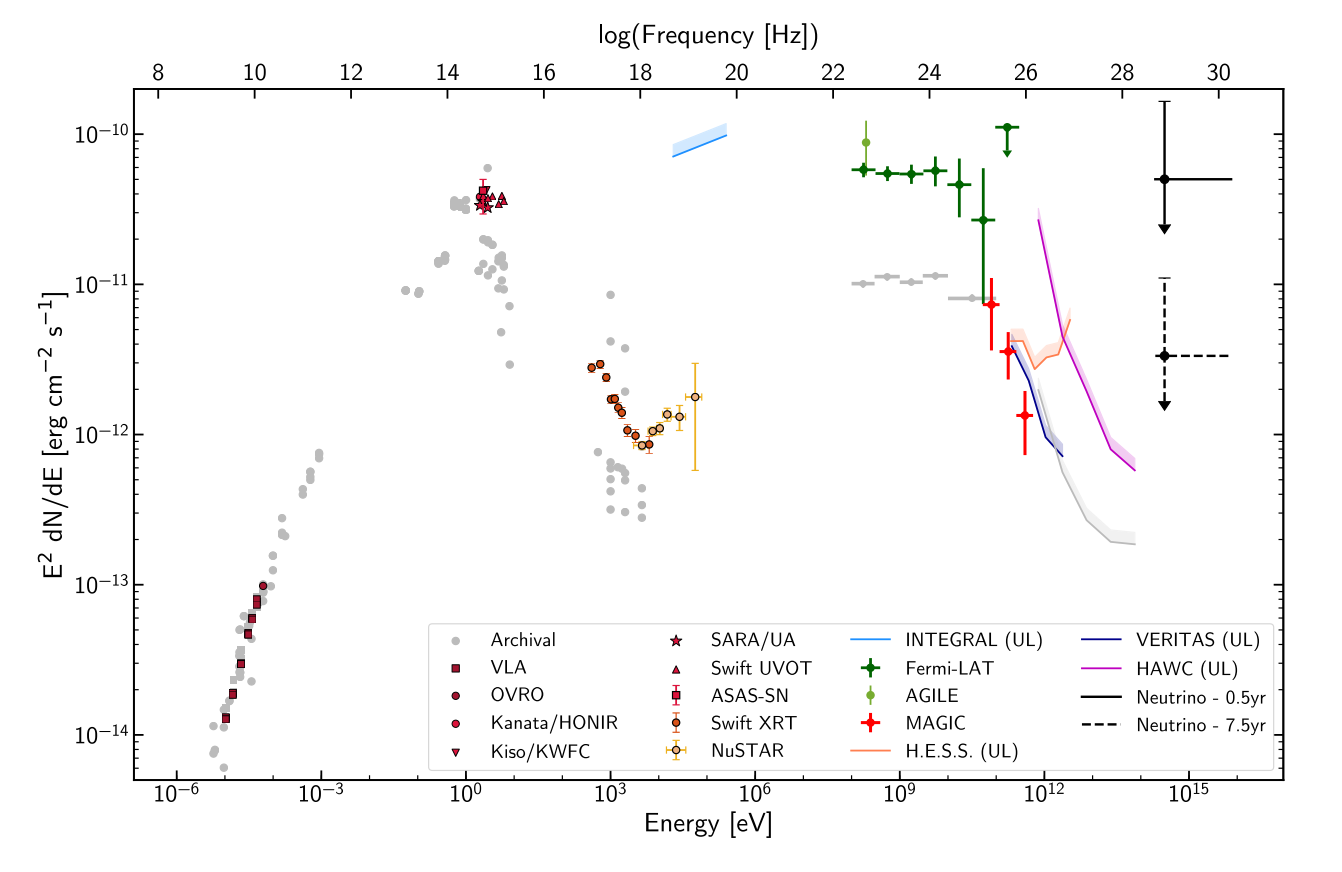
\includegraphics[width=0.7\linewidth]{icecube_spectrum}
  \caption{The broadband spectral energy distribution for the blazar TXS $0506$+$056$ \cite{Ackermann2018} within $14$ days of the detection of the $290\,\textrm{TeV}$ neutrino event. Note in particular that an $E^2 \ud N/\ud E$ scale is equivalent to the more common $\nu F_\nu$ labelling. We will be interested in the pink curve from the HAWC experiment as well as the $0.5$ year neutrino spectrum.}
  \label{fig:spectrum}
  \end{framed}
\end{figure}
Referring to $1.2$ in \cite{dermer2009high}, we start by considering the flux density $F_\nu$, which implies that $\nu F_\nu$ is an energy flux, denoted $\Phi$. Now, we define the luminosity distance $d_L$ which in this case is the comoving distance to the blazar, $\sim 1.3 \, \textrm{Gpc}$. The energy flux is then related to the luminosity $L$ via;
\begin{equation}
  \Phi = \frac{L}{4\pi d_L^2}
\end{equation}
Finally, we define $f_\epsilon := \nu F_\nu$ as a function of the energy. The \textit{luminosity} radiated by a source between energies $\epsilon_1$ and $\epsilon_2$ is then simply;
\begin{equation}
  L[\epsilon_1, \epsilon_2] = 4\pi d_L^2 \int_{\log \epsilon_1}^{\log \epsilon_2}{\upd{\log\epsilon}f_\epsilon}
\end{equation}
So in order to calculate the luminosity of the sources, we need to numerically integrate the curves in Figure \ref{fig:spectrum}.
\subsection{The Numerical Integration}
We are interested in the highest possible energy range possible for the photons given in Figure \ref{fig:spectrum}. Fermi-LAT is sensitive in the region $2\,\textrm{GeV}$ - $1 \, \textrm{TeV}$ \cite{Padovani2018}, however we wish to constrain $\mathcal{O}(100\,\textrm{TeV})$ neutrinos. As such we turn to HAWC. To do the integration, we use a very simple implementation of the trapezium rule;
\begin{equation}
\int_a^b{\upd{x}f(x)} \simeq \sum_{k = 1}^N{\left(f(x_k) + f(x_{k - 1})\right)\Delta x_k}
\end{equation}
where we sample at $a = x_0, x_1, \cdots, x_N = b$, and $\Delta x_k = x_{k} - x_{k - 1}$. We also extract a finite number of points from the curve shown in Figure \ref{fig:spectrum} using \href{https://apps.automeris.io/wpd/}{https://apps.automeris.io/wpd/}. We obtain the numerical results shown in Table \ref{tab:luminosity}. We see there are some discrepancies in that (i) the energy range is lower for the $\gamma$-ray source, and, (ii) the luminosity differs by a factor of $10$. Nonetheless, this is still an improvement on \cite{Kellya, Padovani2018} who both use only Fermi-LAT to obtain the $\gamma$ ray luminosity. As such, for our purposes, the analysis presents a much stronger case and could be improved by extending a best fit curve to the HAWC data to probe higher energies. In terms of motivating the use of the comoving distance as a lower bound on the mean free path, this is a sufficient illustration that the luminosities are indeed similar and so we proceed.
\begin{table}[h]
\centering
\begin{framed}
\begin{tabular}{p{3.0cm}p{3cm}p{5.0cm}p{4.0cm}}
\toprule \textbf{Source} & \textbf{Energy Range} & \textbf{Integrated Flux} $\text{erg}\, \text{cm}^{-2}\,\text{s}^{-1}$ & \textbf{Luminosity} $\text{erg}\,\text{s}^{-1}$\\
\midrule
\textit{$\gamma$ Source (HAWC)} & $0.8 \, \textrm{TeV}$ - $74.0 \, \textrm{TeV}$ & $2.0 \times 10^{-11}$ & $4.1 \times 10^{45}$ \\
\textit{Neutrino Source} & $186 \, \textrm{TeV}$ - $7.9 \, \textrm{PeV}$ & $1.9 \times 10^{-10}$ & $3.8^{+8.5}_{-2.2} \times 10^{46}$ \\
\bottomrule
\end{tabular}
\caption{Numerical Results for the luminosity in the given energy range for the $\gamma$-ray and neutrino components of the blazar flux.}
\label{tab:luminosity}
\end{framed}
\end{table}
\section{Cross-Sections, Channels, and Redshift}
Whilst the cross-section is obviously related to the mean free path, this section deals with some of the assumptions that we make when we model the situation. We will discuss (i) the mass splitting of the scalar spectrum in the scalar case, and, (ii) why we don't need to consider a number of other possible neutrino interactions.
\subsection{Why we Only Need One Process}
In the report detailing how to do the calculation for $\nu\nu \rightarrow \delta\delta$, we neglected to calculate the cross section for other processes within the model that may also lead to a neutrino interaction. These additional processes are as follows;
\begin{enumerate}
  \item \textit{$\nu\nu \rightarrow NN$:} This is less obvious, and indeed one can construct scenarios in parameter space where this dominates. However the centre of mass energy: $E_{\mathrm{com}} = \sqrt{2 E_\nu m_\nu}$ where $m_\nu$ is the mass of the cosmic neutrino background neutrino, is close to the mass of the lightest scalar $\delta$. By construction if the scalar is the dark matter candidate, then the mass of $N$, $m_N$, must be larger. Thus, even in scenarios where the centre of mass energy is large enough to produce two $N$ particles, the cross section is likely to lie at the front tail of the distribution and so be subdominant.
  \item $\nu N \rightarrow \nu N$: There is an $s$-channel and a $t$-channel diagram for this process. Independent of this however, we have assumed that $N$ is not the dark matter candidate. As such, we expect the relic density to be very low in comparison to all other particles. The vertex structure ensures that we expect the cross section to be of a similar order of magnitude to the $\nu\nu \rightarrow \delta\delta$ case. Hence, the contribution to the mean free path is negligible.
  \item $\nu\delta \rightarrow \nu\delta$: It is not immediately clear as to whether this will be negligible. Firstly, there is a $t$-channel process that will have the same algebraic cross section as previously calculated. There is also an $s$-channel process, whose cross-section we obtain from \cite{Franarin2018}. Secondly, we must check the contribution to the mean free path in two regiemes;
  \begin{itemize}
    \item On a cosmological scale where $n_\delta$ is given by the relic density of dark matter,
    \item On a galactic scale, where the density is much higher within the dark matter halo.
  \end{itemize}
\end{enumerate}
Note that neglecting these processes is of course a simplifying assumption about the nature of the cross-sections, but they do not affect the interpretation of the results. This is because including any of the additional contributions above can only \textit{improve} the bounds; for a given $\ell$, introducing a new process increases the effective cross section, and reduces the mean free path leading to tighter constraints.
\subsection{Contribution from $\nu\delta \rightarrow \nu\delta$}
As mentioned above, we must check whether the $\nu\delta \rightarrow \nu\delta$ process contributes significantly to the mean free path of the blazar neutrino. In what follows, we will find that it does not contribute significantly. This is due to the fact that, even within the galactic halo, the cross-section is too small to generate a significant contribution.
\subsubsection{$t$-Channel Cross Section}\label{sec:tchannel}
In the case that the neutrinos are assumed to be massless within the cross-section calculation, we have $\sigma(\nu\nu \rightarrow \delta\delta) \simeq \sigma_t(\nu\delta \rightarrow \nu\delta)$. To see why this is the case, note;
\begin{itemize}
  \item Exchanging $\nu$ and $\delta$ in the initial and final states simply changes the momentum $p_2$ to $p_4$, since the neutrino spinor will now depend on this final state momenta.
  \item This in turn exchanges the factor $(p_1 \cdot p_2)$ with $(p_1 \cdot p_4)$. In the massless neutrino case, we can relate this to the Mandelstam variable, $u$, via $2(p_1 \cdot p_4) = u$.
  \item The relation $u = m_\delta^2 - \tfrac{1}{2}s - \sqrt{s(\tfrac{1}{4}s - m_\delta^2)}\cos\theta$, with $s = \mO(\textrm{GeV})$ ensures that $\Abs{u} \simeq \Abs{s}$ at this energy scale.
\end{itemize}
With these points in mind, at this energy scale, the cross-sections are therefore approximately equivalent, especially at an order of magnitude level. To compare the two cross-sections then, we simply need to evaluate the original cross-section at the centre of mass energy of the $\nu\delta$ collision. This is given by;
\begin{equation}
  \sqrt{s} \simeq \sqrt{2E_\nu m_\delta} \simeq \sqrt{2 \cdot 290 \, \textrm{TeV} \cdot 10\, \textrm{MeV}} \simeq \mO(10 \, \textrm{GeV})
\end{equation}
For an explicit comparison, we put in the values $g_e = 3 \times 10^{-3}$, $g_\mu = 10^{-2}$, $g_\tau = 3\times 10^{-1}$, $m_\delta = 0.5 \, \textrm{MeV}$, $m_\nu = 0.15 \, \textrm{eV}$, $m_N = 5\,\textrm{MeV}$. We find;
\begin{equation}
  \sigma(\nu\nu \rightarrow \delta\delta) \simeq 4.7\times 10^{-10} \, \textrm{MeV}^{-2}, \quad \sigma_t(\nu\delta \rightarrow \nu\delta) \simeq 6.2\times 10^{-16}\, \textrm{MeV}^{-2}
\end{equation}
So we find there is a difference of five to six orders of magnitude. After computing the number density of the dark matter in the galactic and cosmological cases, we will use this to deduce that the $t$-channel does not contribute.
\subsubsection{$s$-Channel Cross Section}\label{sec:schannel}
We obtain an analytic expression for the $s$-channel cross-section from \cite{Franarin2018};
\begin{equation}
  \sigma_s(\nu_\mu\delta \rightarrow \nu_\ell \delta) = \frac{g_\mu^2 g_\ell^2}{16\pi}\frac{(m_N^2 - m_\delta^2)^2}{m_N^2 + m_\delta^2} \frac{1}{(s - m_N^2)^2 + \Gamma_N^2 m_N^2}
\end{equation}
where $\Gamma_N$ is the width of $N$, it is given by;
\begin{equation}\label{eq:sigma_s}
  \Gamma_N = \sum_{\ell}{\frac{g_\ell^2}{16\pi} \frac{(m_N^2 - m_\delta^2)^2}{m_N^3}}
\end{equation}
In this case, we simply do an order of magnitude estimate with;
\begin{equation}
  m_N = \mO(\textrm{MeV}), \quad m_\delta = \mO(\textrm{MeV}), \quad s - m_N^2 = \mO(\textrm{GeV}^2), \quad g = \mO(10^{-2})
\end{equation}
We note that this implies that $(s - m_N^2)^2 \gg \Gamma_N^2 m_N^2$. Putting these into \eqref{eq:sigma_s}, we find;
\begin{equation}
  \sigma_s(\nu\delta \rightarrow \nu\delta) \simeq \mO(10^{-21}\,\textrm{MeV}^{-2})
\end{equation}
As such we deduce that the contribution is certainly negligible at this energy, since even if the number density of $\delta$ was high enough, the $t$-channel process will dominate by $4$ or $5$ orders of magnitude. It therefore remains to check the number density in the cosmological and galactic cases and compare them to the $t$-channel cross-section.
\subsubsection{Number Density on Cosmological Scales}
The dark matter density on a cosmological scale, at a redshift $z$, is given by \cite{Farzan2014};
\begin{equation}
  n(z) = \frac{\Omega_{\textrm{DM},0}\rho_c}{m_{\textrm{DM}}}(1 + z)^3 \simeq 1.26 \times 10^{-3} (1 + z)^3 \left(\frac{\textrm{MeV}}{m_{\textrm{DM}}}\right) \, \textrm{cm}^{-3}
\end{equation}
where we have used $\Omega_{\textrm{DM},0} \simeq 0.265$ and $\rho_c = 3H_0^2/8G \simeq 4.77\, \textrm{keV}\,\textrm{cm}^{-3}$. This is $5$ orders of magnitude below the cosmic neutrino background number density. So in order to be relevant, $\sigma(\nu\delta \rightarrow \nu\delta)$ would have to be approximately $10^5$ times larger than $\sigma(\nu\nu \rightarrow \delta\delta)$, evaluated at the neutrino energy. From Sections \ref{sec:tchannel} and \ref{sec:schannel}, we see this is not the case, and indeed the cross-section is significantly smaller than the $\nu\nu \rightarrow \delta\delta$ cross-section.
\subsubsection{Number Density on Galactic Scales}
After deducing that the contribution to the mean free path is negligible on cosmological scales, we just have to check whether the galactic overdesnity could lead to a significant contribution. As in \cite{Franarin2018}, we use the Einsasto profile with $\alpha = 0.15$ and $R_0 = 20\,\textrm{kpc}$ to model the dark matter energy density;
\begin{equation}
  \rho_{\textrm{DM}}(r) = 7.2 \times 10^{-2}\,\textrm{GeV} \, \textrm{cm}^{-3}\, \cdot \exp\left(-\frac{2}{\alpha}\left(\left(\frac{r}{R_0}\right)^\alpha - 1\right)\right)
\end{equation}
We can obtain the number density by dividing by the mass of the dark matter particle, $m_\delta \simeq \mO(10^{-3} \, \textrm{GeV})$. Now, note that this is maximal when $r = 0$. In order to put an upper bound on the contribution to the mean free path, we assume that the whole halo has this maximal number density. With $m_\delta = 1\, \textrm{MeV}$;
\begin{equation}
  n_{\textrm{DM}}^{\textrm{max}} \simeq \frac{\rho_{\textrm{DM}}(r = 0)}{m_\delta} \simeq 4.4 \times 10^{7} \, \textrm{cm}^{-3} \simeq 10^{5} n^0_{\nu}
\end{equation}
Now we are in a position to see why this does not contribute to the suppression of the neutino flux from the blazar. Whilst the combination of $n^{\textrm{max}}_{\textrm{DM}} \sigma_t(\nu\delta\rightarrow\nu\delta)$ is now of the same order of magnitude as $n_\nu \sigma(\nu\nu\rightarrow \delta\delta)$, the relevant consideration is the probability that such an interaction ($\nu\delta \rightarrow \nu\delta$) occurs. This is dependent on the ratio between the length scale at which such a high number density is observed (i.e. the galactic radius), and the mean free path. Here, the mean free path is $\mO(\textrm{Gpc})$, so the probability of such an interaction occuring is $\sim \exp(-d_{g}/\mO(\textrm{Gpc}))$ where $d_g = \mO(\textrm{kpc})$ is the galactic radius. We see that this is negligble. Finally, note that in the case where the mean free path is $\mO(\textrm{kpc})$, we would not expect the neutrino to reach anywhere close to the galaxy, so this would be inconsequential also. Hence we deduce that both in the cosmological and galactic settings, the contribution from $\nu\delta \rightarrow \nu\delta$ is negligible in comparison to the dominant $t$-channel process $\nu\nu \rightarrow \delta\delta$.

To end this section, we emphasise that whilst we have neglected the contribution from these other processes, including any/all of them can only improve the bounds as the mean free path will decrease with new interactions. As such, it is only for the sake of simplicity that we make the assumptions, \textit{not} at the cost of the validity of the bounds.
\subsection{Mass Splitting and a Factor of Three}
Within the code for the project, we assume that each of the mass eigenstates is equally abundant $\nu_1, \bar{\nu}_1, \nu_2, \ldots$, with a number density given by;
\begin{equation}
  n_{\nu_i} = \frac{1}{6} n_\nu = \frac{1}{6} \cdot 340 \, \textrm{cm}^{-3}
\end{equation}
Now, the contribution from each mass eigenstate to the inverse mean free path $\ell^{-1}$ is given by $n_{\nu_i} \sigma(\nu_\mu X \rightarrow Y )$. Importantly we argued in the last section that we thus need only consider $\sigma(\nu_\mu \nu \rightarrow \delta \delta)$. Now, in the real case, there is nothing more to say as there is only one scalar mass eigenstate. In the complex case however, we must consider the following. The theory we are considering is effective up to some scale $\Lambda$. It therefore does not have to explicitly respect any of the symmetries that might apply in the UV. Indeed all we assume is that the new dark sector particles are odd under a $\mathbb{Z}_2$ symmetry, to ensure there is a stable candidate. As such, writing $\delta = \tfrac{1}{\sqrt{2}}(\delta_1 + i \delta_2)$, the most general hermitian mass term can be written;
\begin{equation}
  V_m = M^2 \delta\dagg \delta - \frac{1}{2}(m^2 \delta \delta + \textrm{h.c.})
\end{equation}
This leads to a mass splitting between the mass eigenstates $\delta_{1,2}$ given by $\Delta m_{12}^2 = 2m^2$. Now, we consider the possible processes $\nu\nu \rightarrow \textrm{scalars}$. We have;
\begin{equation*}
\nu\nu \rightarrow \delta_1 \delta_1, \quad \nu\nu \rightarrow \delta_1 \delta_2, \quad \nu\nu \rightarrow \delta_2 \delta_2
\end{equation*}
From this we see that there are a couple of scenarios that might occur kinematically. We assume that the lightest scalar is $\delta_1$, and that the first process can happen. Then it may the case that either (i) only the first process can occur, (ii) only the first and second processes can occur, or, (iii) all the processes can occur. This is where we make our simplifying assumption, which unlike the first case, will not necessarily improve the bounds if put in at a later date. We assume that if the first occurs, then the next two may also occur. This is equivalent to saying that there is a small mass gap between the two eigenstates. A priori, without a UV theory, the mass parameter, $m$, is somewhat arbitrary. To simplify the situation then we assume that $m$ is small compared to $M$, and therefore that we can approximate;
\begin{equation}
  \sigma(\nu\nu \rightarrow \delta_1 \delta_1) + \sigma(\nu\nu \rightarrow \delta_1 \delta_2) + \sigma(\nu\nu \rightarrow \delta_2 \delta_2) \simeq 3 \sigma(\nu\nu \rightarrow \delta_1 \delta_1)
\end{equation}
\subsection{Redshift}
During the cosmological propagation, both the number density of the cosmic neutrino background neutrinos, and the energy of the blazar neutrino will be affected by redshift. Let the values now be denoted $n_\nu^0$ and $E_\nu^0$ respectively, then at a redshift $z$;
\begin{equation}
  n_\nu(z) = n_\nu^0 (1 + z)^3, \quad E_\nu(z) = (1 + z)E_\nu^0
\end{equation}
We now make the observation that the source of the $290 \, \textrm{TeV}$ neutrino is at a redshift $z = 0.3365$. In the case of the energy this means that the maximum possible multiplicative factor is $(1 + 0.3365)$, but this is within the confidence bounds on the energy measured at IceCube, so can be neglected. The redshift of the number density is not negligible however, although it only improves the bounds. We take the result from \cite{Farzan2014} that the optical depth is given by;
\begin{equation}
  \tau = c\int_{z = z_1}^{z = z_2}{\upd{z}\frac{\ud t}{\ud z}n(z)\sigma(z)}
\end{equation}
With the assumption above that $E_\nu(z)$ does not appreciably depend on the redshift, this reduces to;
\begin{equation}
  \tau = c n_\nu^0 \sigma(E_\nu^0) \int_{z = z_1}^{z = z_2}{\upd{z}(1 + z)^3 \frac{\ud t}{\ud z}}
\end{equation}
We can relate $\ud t/\ud z$ to the Hubble rate via;
\begin{equation}
  \frac{\ud t}{\ud z} = -\left((1 + z)H(z)\right)^{-1}
\end{equation}
where;
\begin{equation}
  H(z) = H_0 \sqrt{\Omega_\Lambda + \Omega_{m,0}(1 + z)^3}
\end{equation}
We will take the values $\Omega_\Lambda \simeq 0.65$, $\Omega_{m,0} \simeq 0.315$, $H_0 \simeq 6.73 \times 10^{4}\, \textrm{km}\,\textrm{s}^{-1}\textrm{Gpc}^{-1}$, $c = 3\times 10^{5}\,\textrm{km s}^{-1}$. Letting $\ell_0^{-1} := n_\nu^0 \sigma(E_\nu^0)$ to find;
\begin{equation}
  \tau = \left(\frac{\ell_0}{\text{Gpc}}\right)^{-1} \left(\frac{c \, / \, \text{km s}^{-1}}{H_0 \, /\, \text{km s}^{-1}\text{Gpc}^{-1}}\right) \cdot \int_{z = z_1}^{z = z_2}{\upd{z}\frac{(1 + z)^2}{\sqrt{\Omega_\Lambda + \Omega_{m,0}(1 + z)^3}}} \simeq 1.90 \left(\frac{\ell_0}{\textrm{Gpc}}\right)^{-1}
\end{equation}
\section{Including Neutrino Mass Hierarchies}
The last technicalities to introduce into the computation of the bounds are the facts that;
\begin{enumerate}
  \item The neutrino \textit{mass} eigenstates and \textit{flavour} eigenstates are not simultaneous
  \item The neutrino masses are unknown, and indeed have two possible orderings (for the mass eigenstates); the \textit{normal hierarchy} and the \textit{inverted hierarchy}.
\end{enumerate}
Within our calculation we aim to present the situation for both of these cases.
\subsection{Mass Eigenstates and the PMNS Matrix}
Neutrinos are neutral (i.e. lie in the trivial representation) under the Standard Model gauge group, and therefore cannot couple to the Higgs doublet in a gauge invariant way. Therefore within the Standard Model, we expect them to be massless. Experiments illustrating phenomena such as neutrino oscillations contradict this fact and we now believe they do indeed have a small mass. This complicates matters however for the reason mentioned above. The flavour eigenstates and the mass eigenstates are no longer simultaneous in this case. Instead they are related by the \textit{PMNS} matrix\footnote{Pontecorvo-Maki-Nakagawa-Sakata}. This encodes a unitary transformation between the flavour basis and the mass basis:
\begin{equation}
  \mathbf{\nu}_\ell := \begin{pmatrix} \nu_e \\ \nu_\mu \\ \nu_\tau \end{pmatrix} = \thrbythr{U_{e1} & U_{e2} & U_{e3}}{U_{\mu1} & U_{\mu2} & U_{\mu3}}{U_{\tau1} & U_{\tau2} & U_{\tau3}} := U \mathbf{\nu}_i
\end{equation}
We can parametrise the PMNS matrix as;
\begin{equation}
  U = \thrbythr{c_{12}c_{13} & s_{12}c_{13} & s_{13}e^{-i\delta_{\textrm{CP}}}}{-s_{12}c_{23} - c_{12}s_{23}s_{13}e^{i\delta_{\textrm{CP}}} & c_{12}c_{23} - s_{12}s_{23}s_{13}e^{i\delta_{\textrm{CP}}} & s_{23}c_{13}}{s_{12}s_{23} - c_{12}c_{23}s_{13}e^{i\delta_{\textrm{CP}}} & -c_{12}s_{23} - s_{12}c_{23}s_{13}e^{i\delta_{\textrm{CP}}} & c_{23}c_{13}}
\end{equation}
where $c_{12} = \cos\theta_{12}, s_{13} = \sin\theta_{13}$ etc. and;
\begin{equation}
  \theta_{12} = 33.63^{+0.78}_{-0.76}\deg, \quad \theta_{23} = 47.2^{+1.9}_{-3.9}\deg, \quad \theta_{13} = 8.54^{+0.15}_{-0.15}\deg, \quad \delta_{\textrm{CP}} = 234^{+43}_{-31}\deg
\end{equation}
With this formalism in place, we can then relate for example, the masses of the flavour eigenstates to those of the mass eigenstates;
\begin{equation}
  m_{\nu_\ell}^2 = \sum_{i}{\Abs{U_{\ell i}}m_{\nu_i}^2}
\end{equation}
\subsection{The Mass Hierarchy}
A key fact in this discussion is that ultimately we do not know the absolute values, nor the ordering of the mass eigenstates. There are two common alternatives, which are illustrated in Figure \ref{fig:hierarchy} from \cite{King};
\begin{figure}[h]
  \begin{framed}
  \centering
  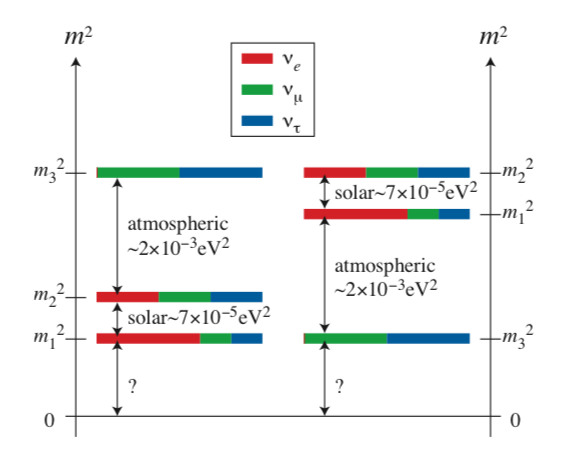
\includegraphics[width=0.5\linewidth]{mass_hierarchy}
  \caption{The possible options for the neutrino mass hierarchy, \textbf{Left:} the normal ordered hierarchy where two neutrinos are light and $\nu_3$ is heavier, \textbf{Right:} the inverted hierarchy where $\nu_3$ is light and $\nu_{1,2}$ are heavier.}
  \label{fig:hierarchy}
  \end{framed}
\end{figure}
\begin{enumerate}
  \item \textit{Normal Ordering:} In the normal hierarchy, $\nu_3$ is the most massive state, whilst $\nu_1$ and $\nu_2$ are lighter.
  \item \textit{Inverted Ordering:} On the other hand, in the inverted case, $\nu_3$ is the lightest, whilst $\nu_1$ and $\nu_2$ are heavier.
\end{enumerate}
\subsection{Constraints on the Masses}
We can go slightly further, whilst we do not know the precise masses of the neutrinos we have (i) a bound on the total sum of the masses that comes from Cosmology, and, (ii) values for the mass difference between the eigenstates, as illustrated in Figure \ref{fig:hierarchy}. To be more precise;
\begin{itemize}
  \item Combining constraints from Cosmic Microwave Background (CMB) anisotropies, Baryon Acoustic Oscillations, Type 1A Supernovae, and, CMB lensing, we will use the constraint \cite{Couchot2017};
  \begin{equation}
    \sum{m_{\nu_i}} < 0.17 \, \textrm{eV}
  \end{equation}
  \item We also know the squared mass differences between some of the mass eigenstates \cite{Couchot2017};
  \begin{align}
    \Delta m_{12}^2 = m_2^2 - m_1^2 &= 7.37 \times 10^{-5}\,\textrm{eV}^2 \\
    \Delta m^2 = m_3^2 - \frac{1}{2}(m_1^2 + m_2^2) &= +2.50 \times 10^{-3} \, \textrm{eV}^2\, \textrm{(NH)} \\
    &= -2.46 \times 10^{-3} \, \textrm{eV}^2\, \textrm{(IH)}
  \end{align}
\end{itemize}
From the last of these constraints we see that fixing one of the masses automatically fixes the others. In our analysis we intend to vary one of the masses of the mass eigenstates and use the squared mass differences to compute the other masses, remaining within the bound set by the cosmological considerations. We will present the analysis in both the normal and inverted cases.
\subsection{The Coupling Constants}
There is one final consequence of the non-coincidence of the mass and flavour eigenstates. We are considering a coupling in the Lagrangian of the form;
\begin{equation}
  \mL_{\textrm{new}} = \sum_{\ell}{g_\ell \delta \bar{N}_R \nu_{\ell, L} + \textrm{h.c.}}
\end{equation}
where importantly, the $\nu_{\ell}$ are the flavour eigenstates. Furthermore, we quoted constraints on the couplings $g_\ell$ in this flavour basis e.g. $g_{\ell} < 10^{-3}$ in the case of real dark matter. Now consider expanding in the mass basis;
\begin{equation}
  \mL = \delta \bar{N}_R \sum_{\ell}{g_\ell \sum_{i}{U_{\ell i}\nu_{i, L}}} + \textrm{h.c.} := \sum_i{g_i \delta \bar{N}_R \nu_{i, L}}
\end{equation}
We have defined the couplings to the neutrino mass eigenstates;
\begin{equation}
  g_i := \sum_{\ell}{U_{\ell i}g_{\ell}}
\end{equation}
Now, importantly, these will inherit constraints from the constraints on the flavour basis couplings, and are just related by a linear transformation. This means that we can still parametrise our constraints in terms of the flavour couplings. The context of these comments is that the cosmic neutrino background consists of decoherent mass eigenstates. Therefore instead of considering flavour processes $\nu_\mu \nu_\ell, \nu_\mu \bar{\nu}_\ell \rightarrow \delta\delta$, we should instead consider $\nu_\mu \nu_i \rightarrow \delta \delta$. To do so we should use the $\set{g_i}$ couplings at the $\nu_i \delta N$ vertex, which we can compute as above. We also make use of the mass eigenstate masses as discussed above to compute the centre of mass energy in each of the different cases $i = 1,2,3$. Finally, we will assume that each of the mass eigenstates is equally abundant in the cosmic neutrino background so that we can take the number density of each species to be $n_\nu/6$ as noted previously.
\section{Neutrino Clustering}
The main reference is \cite{Ringwald2004} which discusses the clustering of cosmic neutrino background neutrinos onto cold dark matter. In the context of this work, this would affect the number density $n_\nu(z)$ as the astrophysical neutrino passed through different dark matter distributions. In regions where there is more cold dark matter, \cite{Ringwald2004} suggests that we should see more cosmic microwave background neutrinos. A precision analysis of the propagation of the neutrinos from the blazar should take this into account.

This being said, \cite{Ringwald2004} only extends the analysis to the local group\footnote{The \textit{Greisen-Zatsepin-Kuzmin} zone}, across distances of $\textrm{Mpc}$. This is ultimately small scale structure in the context of $\textrm{Gpc}$ propagation. Figure 8 in \cite{Ringwald2004} illustrates the density contrast of the neutrinos on this scale. We see that density constrasts of $\mO(2)$ are realistic, so including this effect could strengthen the bounds. This sort of precision analysis is beyond the scope of this work however.
\section{Conclusions}
To conclude this report, we began in a position where we had an explicit calculation of the cross section, and a presentation of the effective field theory along with the constraints on the couplings. We have now attempted to clarify a number of points to fill in the gaps in our analysis. These include;
\begin{enumerate}
  \item A clear description of the parameter values and assumptions regarding the production mechanism of neutrinos within the blazar TXS $0506$+$056$.
  \item More detail regarding the high energy neutrino event on $22$ September $2017$ which we will use to constrain the model.
  \item Justifying our assumption that the mean free path of ultra high energy neutrinos from the blazar should be greater than the distance to the blazar. This was achieved by integrating the flux curves in the $\gamma$-ray, and neutrino cases and comparing their luminosity over relevant energy ranges.
  \item Discussed how to include the effect of redshift on the number density and energy of the neutrinos.
  \item Illustrated some of the subtleties regarding the cross-section in the complex scalar case, and clarifying our assumption that the splitting between the mass eigenstates is small.
  \item Identified a method of including the neutrino mass spectrum within the calculation.
\end{enumerate}
It remains to include these assumptions and improvements within the code to generate the constraints, and then investigate whether suitable bounds still apply.
%\end{multicols*}
\vspace{20pt}
\hrule
\vspace{1pt}
\hrule
\vspace{3pt}
\bibliography{details}
\vspace{15pt}
\hrule
\vspace{1pt}
\hrule
\end{document}
